\documentclass[dvipdfmx,12pt,unicode]{beamer}
\usepackage{graphicx}
\usepackage{amsmath}
\usepackage{amsfonts}
\graphicspath{{./img/}}
\usetheme{CambridgeUS}
\usecolortheme{dolphin}
\setbeamertemplate{footline}[frame number]
\setbeamertemplate{caption}[numbered]
\renewcommand{\figurename}{図}
\renewcommand{\tablename}{表}
\logo{
\includegraphics[width=1cm]{img/logo.png}}

\usefonttheme{professionalfonts}

\title{Parameter Unsharingを用いたMode Collapseの回避}
\author{raven(Kai Katsumata)}
\institute[JPN]{SL B2 \\ 親 ryoga}

\begin{document}

\begin{frame}\frametitle{}
  \maketitle
\end{frame}

\begin{frame}{背景}
  自動運転の研究開発においてデータセットの作成やVirtual EvaluationなどでGAN\cite{gan}が用いられることが増えてきた。
  \begin{figure}[htb]
    \centering    
    \includegraphics[width=\linewidth]{pix2pixhd.png}
    \caption{pix2pixHD {\scriptsize https://tcwang0509.github.io/pix2pixHD/ より引用}}
  \end{figure}        
\end{frame}

\begin{frame}{背景2}
  \begin{itemize}
  \item 高解像度の町並みの生成\cite{pix2pixhd}
  \item 生成する画像のコントロール\cite{pix2pixhd}
  \item 自動車のシミュレータのリアリスティック化\cite{simgan}
  \end{itemize}
  \begin{figure}[htb]
    \centering    
    \includegraphics[width=7cm]{simgan.png}
    \caption{SimGAN \cite{simgan}より引用}
  \end{figure}          
\end{frame}

\begin{frame}{GANの課題}
  Mode Collapseと呼ばれる現象が発生する
  \begin{figure}[htb]
    \centering
    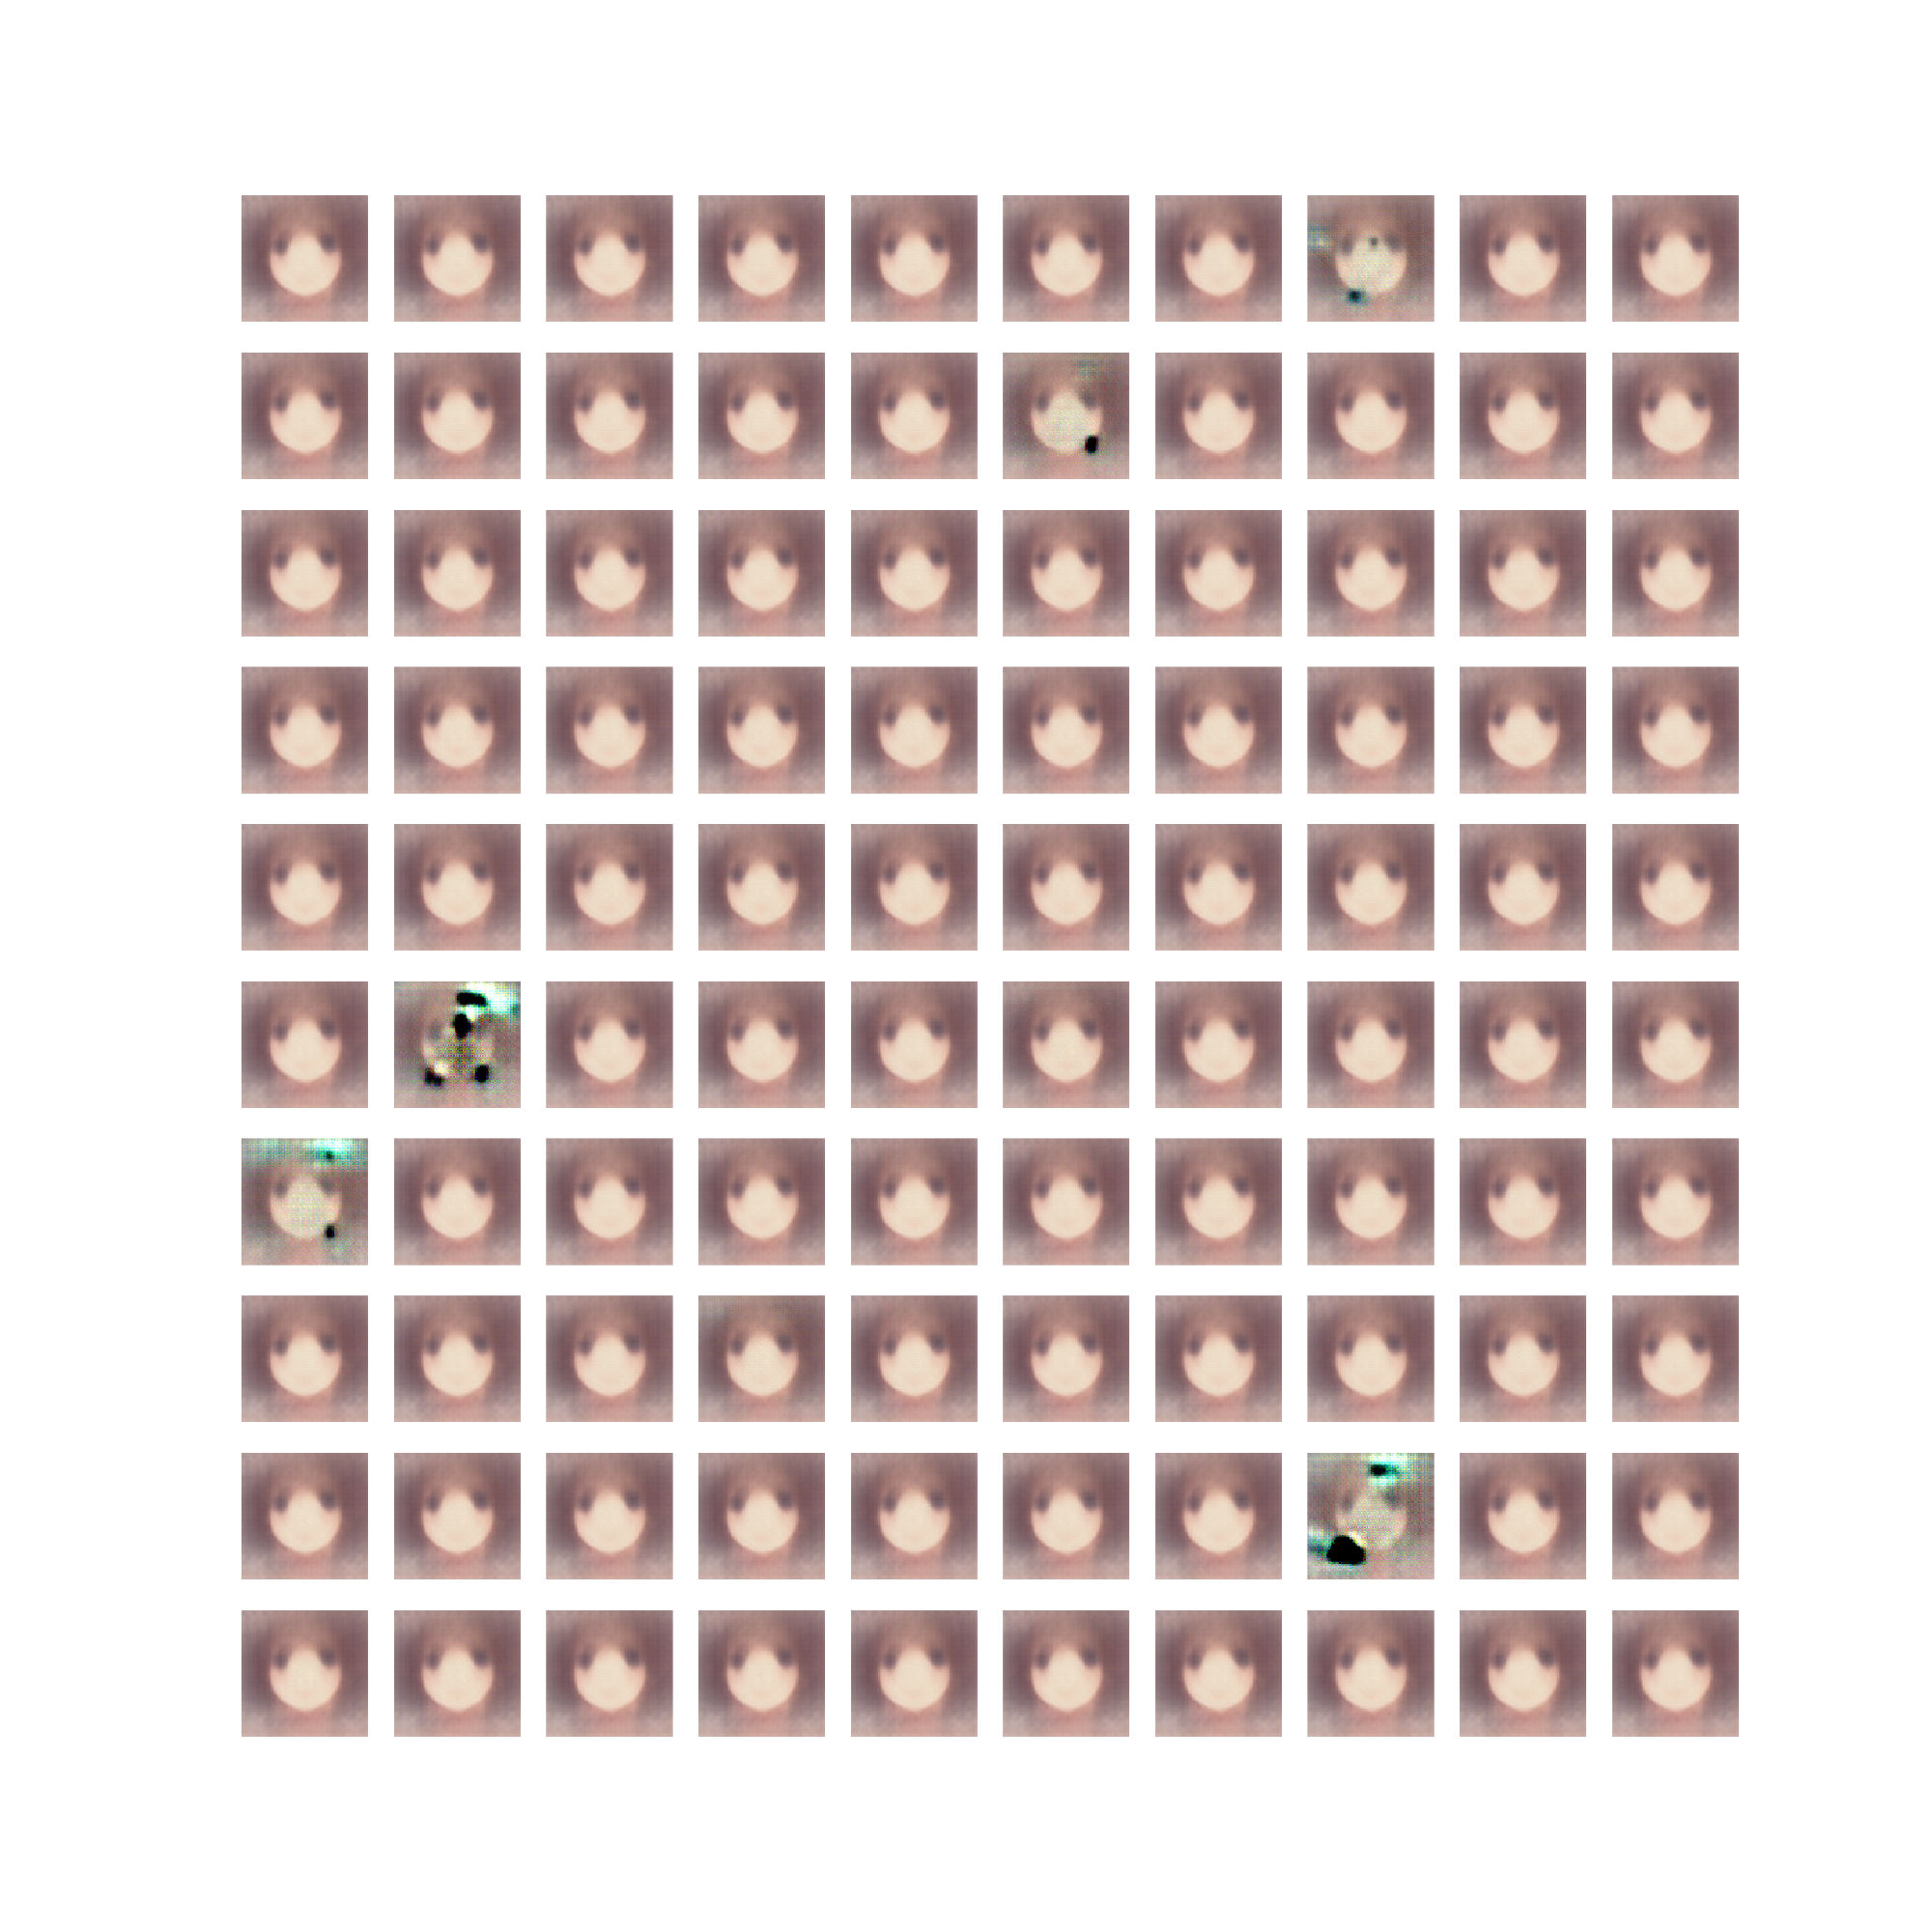
\includegraphics[height=6cm]{collapse.png}
    \vspace*{-1cm}    
    \caption{Collapseの例: {\scriptsize http://musyoku.github.io/2017/04/16/Boundary-Equilibrium-Generative-Adversarial-Networks/ より引用} \label{fig:collapse}}
  \end{figure}  
\end{frame}

\begin{frame}{本研究の目的}
  \begin{itemize}
  \item GANの問題点であるMode Collapseの回避
  \item 多様な表現を出力するGANの生成
  \end{itemize}
\end{frame}

\begin{frame}{関連研究}

  \begin{block}{Unrolled GAN\cite{unrolled}}
    Generatorを未来のDiscrimiantorを騙せるように学習させることでMode Collapseを回避することに成功.
  \end{block}

  \begin{block}{PacGAN\cite{pacgan}}
    Discriminatorが真偽を判定するのに一枚ずつ行っていたのをバッチごとに行うようにした. 分布をより正確に捉えられるようになった.
  \end{block}
\end{frame}

\begin{frame}{既存研究の課題}
  \begin{itemize}
  \item 計算コストが高い(Unrolled GAN)
  \item Semi Supervised Learningで利用ができない(PacGAN)
  \item 一定の解に収束しやすくなる(何回学習をしても同じ表現しか得られない)(Unrolled GAN, PacGAN)
  \end{itemize}
\end{frame}

\begin{frame}{提案手法}
  過去に学習したモデルの重みから遠ざけるように学習させることで
  別の局所最適解を探索させる

  \begin{figure}[htb]
    \centering    
    \includegraphics[width=10cm]{loss.png}
  \end{figure}  
\end{frame}

\begin{frame}{提案手法}

目的関数を

\begin{equation}
  \label{unshare}
  \tilde{\mathcal{L}}(\pmb{w}; \pmb{X}, \pmb{y}, \pmb{w}') =
  -\frac{\alpha}{2} (\pmb{w} - \pmb{w}')^{\top}(\pmb{w} - \pmb{w}') + \mathcal{L}(\pmb{w}; \pmb{X}, \pmb{y})  
\end{equation}


のように定義する
  
\end{frame}

\begin{frame}{実験 1: 多項式フィッテイング}
  $\pmb{X} = \{1, 2, 3, 4, 5,...\}, \pmb{y} = \{4, 16, 36, 64, 100,..\}$. \\
  $\pmb{y} = (2\pmb{x})^{2}$もしくは$\pmb{y} = (-2\pmb{x})^{2}$. \\
  目的関数は
  
  \begin{equation}
    \label{regression}
    \mathcal{L}(\pmb{w}; \pmb{X}, \pmb{y}, \pmb{w}')
    =  -\frac{\alpha}{2} (\pmb{w} - \pmb{w}')^{\top}(\pmb{w} - \pmb{w}') + (f(\pmb{X}) - \pmb{y})^{2} 
  \end{equation}      
\end{frame}

\begin{frame}{実験 2: GAN(混合正規分布)} 
  平均をずらした正規分布の混合分布から生成させたデータを生成させる. 
  2,3,4つの正規分布の混合分布を生成させた. \\
  目的関数は
  
  \begin{equation}
    \begin{split}
    \label{gan}
    \mathcal{L}o(\theta_{G}, \theta_{D}, \theta'_{G})
    & =  -\frac{\alpha}{2} (\theta_{G} - \theta'_{G})^{\top}(\theta_{G} - \theta'_{G})  \\
    & \quad +  \mathbb{E}_{x\sim p_{data}} [ \log(D(x; \theta_{D})) ]    \\ 
    & \quad + \mathbb{E}_{z\sim \mathcal{N}(0, I)} [ \log(1 - D(G(z;\theta_{G}); \theta_{D})) ]
    \end{split}
  \end{equation}        
\end{frame}

\begin{frame}
  \begin{figure}[htb]
    \centering    
    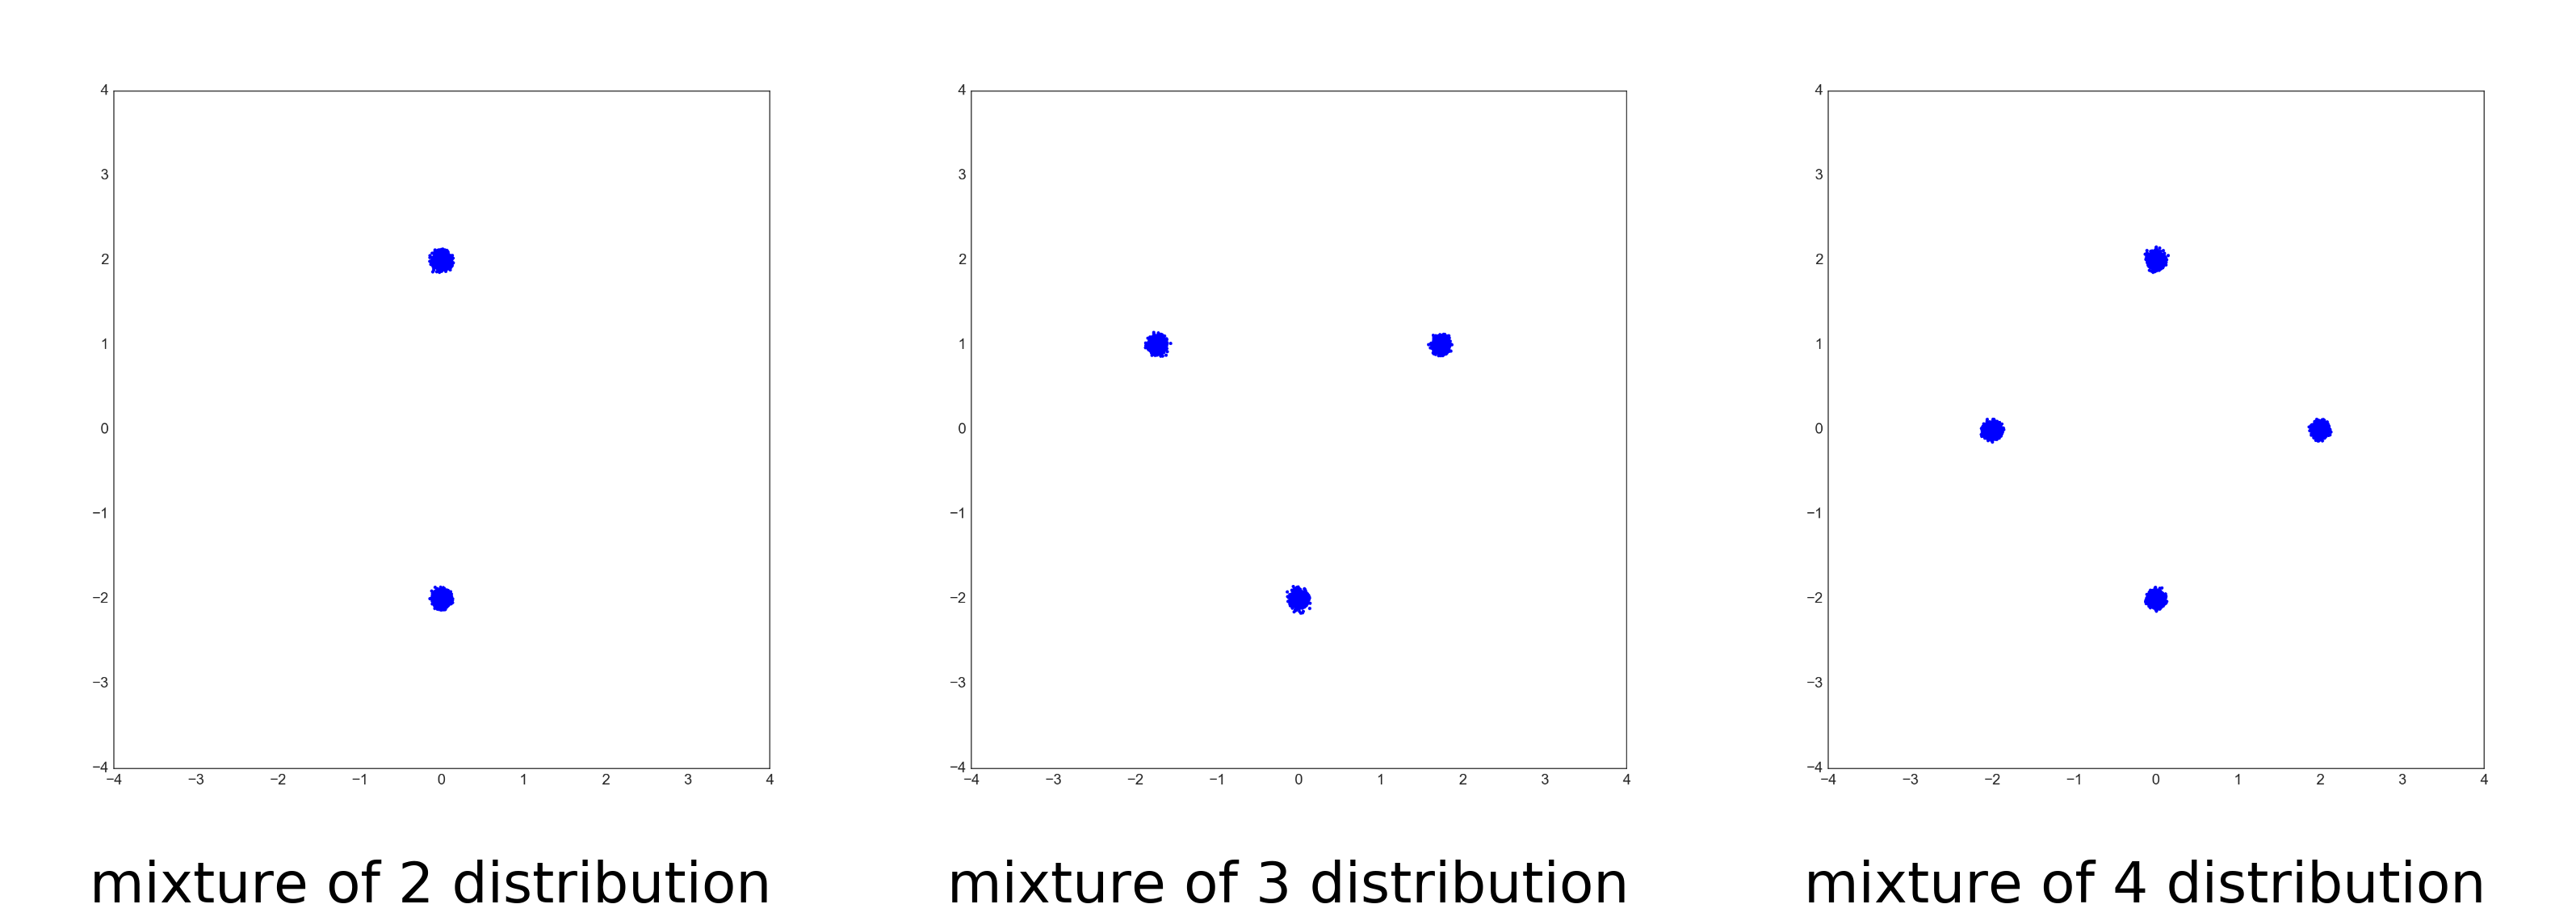
\includegraphics[width=\linewidth]{true.png}
    \caption{再現する混合正規分布}
  \end{figure}
\end{frame}

\begin{frame}{mixture of 2 distribution}
  \begin{figure}[htb]
    \centering        
    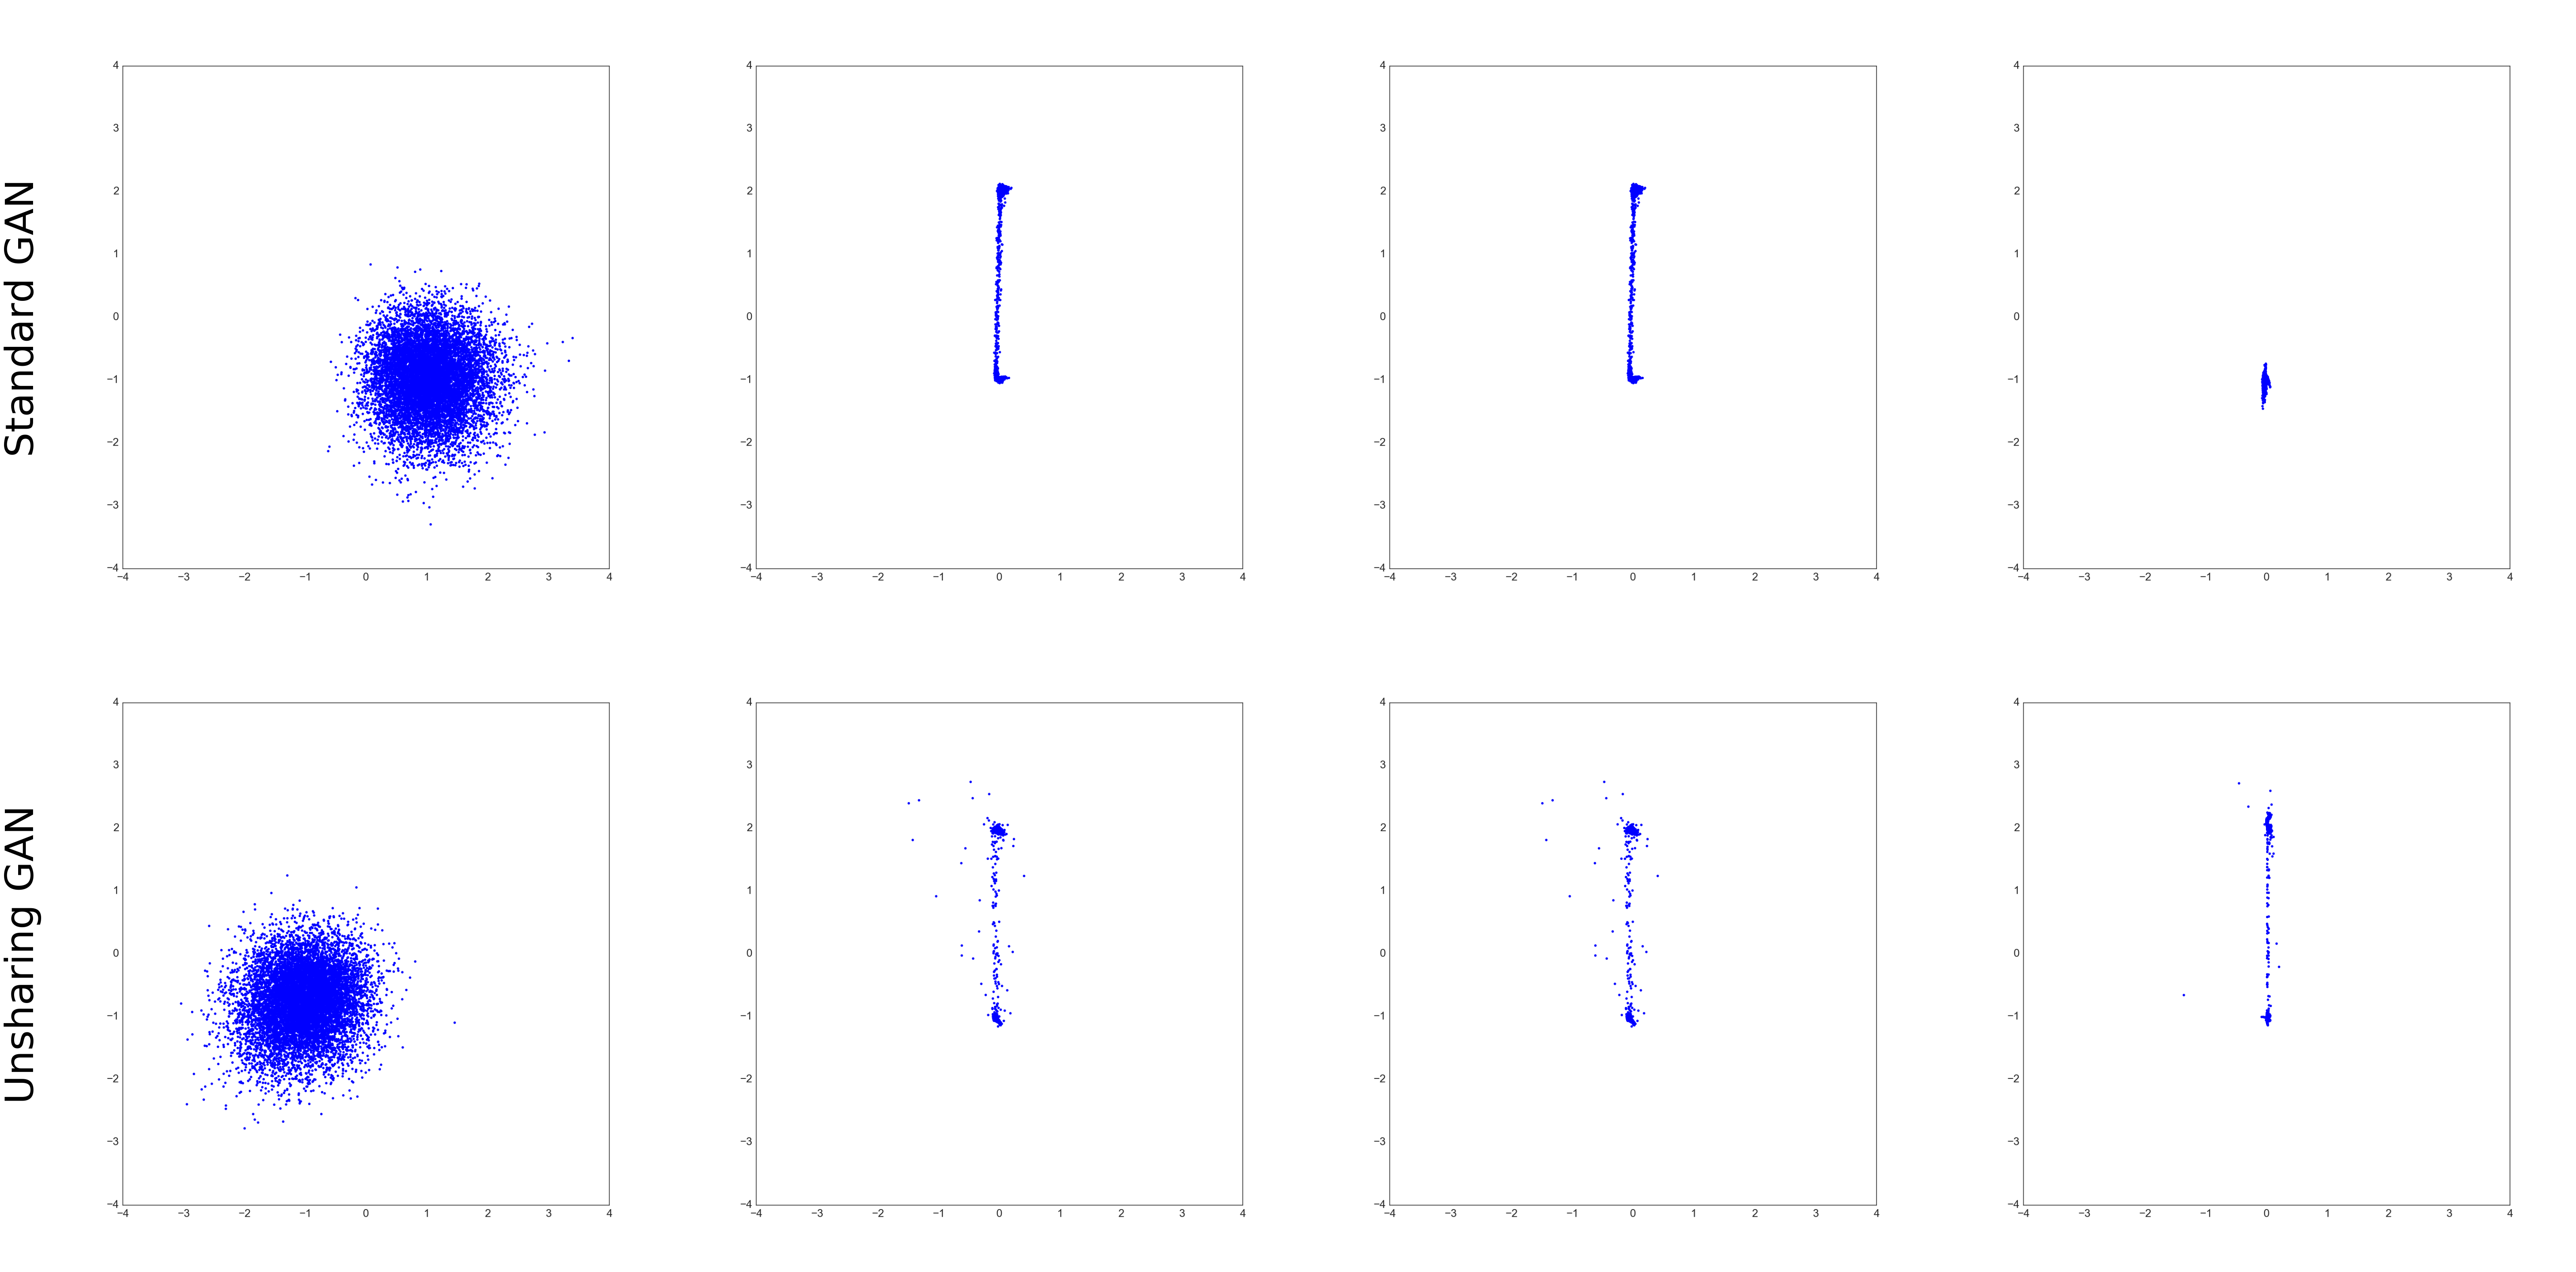
\includegraphics[width=\linewidth]{2_mixture_gan.png}
  \end{figure}
\end{frame}

\begin{frame}{mixture of 3 distribution}
  \begin{figure}[htb]
    \centering    
    \includegraphics[width=\linewidth]{3_mixture_gan.png}
  \end{figure}
\end{frame}

\begin{frame}{mixture of 4 distribution}
  \begin{figure}[htb]
    \centering        
    \includegraphics[width=\linewidth]{4_mixture_gan.png}
  \end{figure}
\end{frame}

\begin{frame}{他手法との組み合わせ}
  \begin{figure}[htb]
    \centering        
    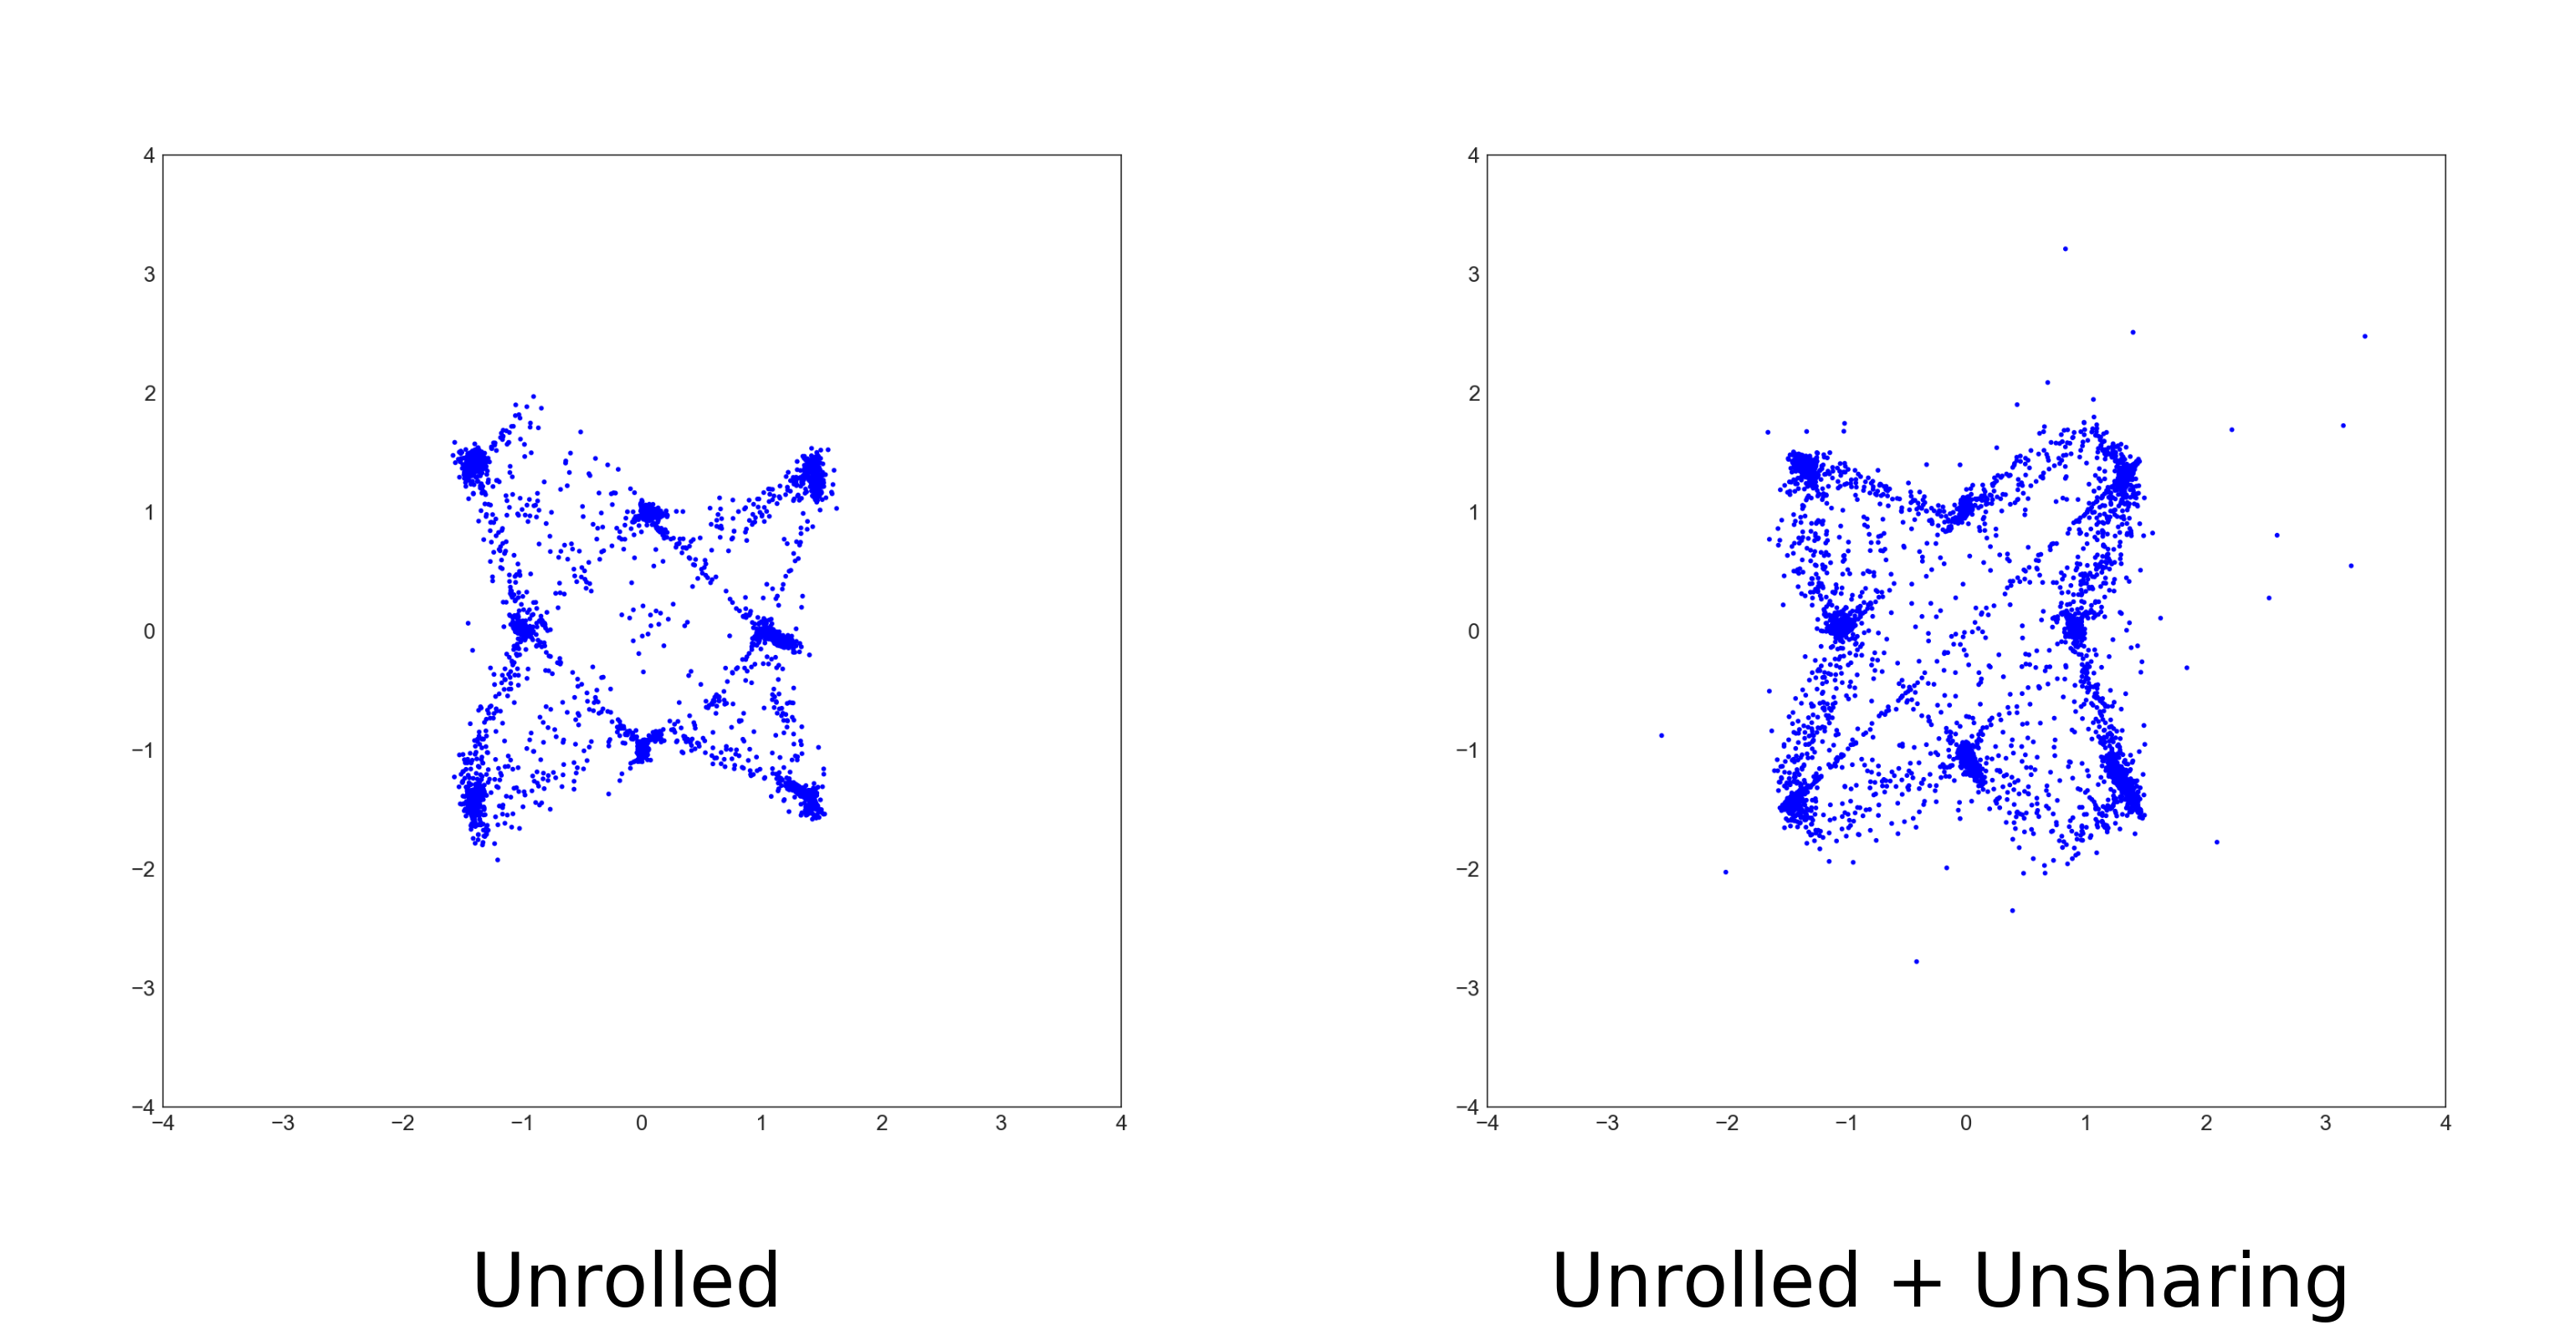
\includegraphics[width=\linewidth]{unrolled.png}
    \caption{Unrolledのみとは少し異なる分布が再現できた}
  \end{figure}
\end{frame}

\begin{frame}{今後の展望}
  \begin{itemize}
  \item 今回はMLP及び単純なGANにおいて提案手法が有効であることを検証したが,
    画像を生成するような複雑なGANでも検証が不十分.
  \item 他の安定化手法との比較が不十分であるため要検証.
  \item 他の安定化手法と組み合わせた際に同様の分布を捉えつつ, 異なる表現を獲得することが確認できた.
    この特性がデータセットの拡充などに利用できるか検証を行う.
  \end{itemize}
\end{frame}

\begin{frame}[allowframebreaks]{参考文献}
  \beamertemplatetextbibitems
\bibliographystyle{jplain}
\bibliography{ref}
\end{frame}

\begin{frame}{Appendix}
  GANの目的関数 \\
  \begin{equation}
    \begin{split}
    \label{gan_main}
    \mathcal{L}o(\theta_{G}, \theta_{D}) & =  \mathbb{E}_{x\sim p_{data}} [ \log(D(x; \theta_{D})) ]    \\ 
    & \quad + \mathbb{E}_{z\sim \mathcal{N}(0, I)} [ \log(1 - D(G(z;\theta_{G}); \theta_{D})) ]
    \end{split}
  \end{equation}
\end{frame}
\end{document}
